\chapter{Diffusion and the scales it finds}
\label{ch:diffusion}

\section{Diffusion, not just drift}

Chapter~\ref{ch:search} put a walker on a network and used it to \emph{grow} one.
The walker was a device: what mattered was how often it landed on a node, because
that set how fast the node acquired links. This chapter puts a walker on the
networks those rules have already built, and asks what it can tell us about them.
It is the same walk. The question is different, and so is the part of the walk that
answers it.

Start with what a random walk forgets, because Chapter~\ref{ch:search} leaned on it
and it is worth being exact about what was borrowed. On a connected network the walk has a unique stationary
distribution, and it is the one Chapter~\ref{ch:search} used,
\begin{equation}
  P^\infty_i = \frac{k_i}{2m},
  \label{eq:hc-stationary}
\end{equation}
reached from any starting point. That distribution knows the degree sequence and
nothing else: two networks with the same degrees are indistinguishable to it. And
the blindness runs a little deeper than the stationary state. The mean time for a
walker to \emph{return} to where it started is
\begin{equation}
  \langle T_{ii}\rangle = \frac{2m}{k_i},
  \label{eq:hc-return}
\end{equation}
exactly, on every connected network \citep{noh2004} --- an identity with no
architecture in it at all. Whether the node sits in a dense community, on a bridge,
or at the end of a long chain does not enter. Only its degree and the size of the
network do.

It would be easy to conclude from those two identities that a classical walk can
report only degrees, and that conclusion is the one thing this chapter most needs to
head off. What is degree-blind is the walk's \emph{stationary} behaviour --- where it
ends up, and how long it takes to come home. How it gets there is not blind at all,
and everything below is an attempt to read it.

\begin{calculation}{first passage times, and what they know}
Let $\langle T_{ij}\rangle$ be the mean number of steps for a walker started at $i$
to first reach $j$. For a connected undirected network this has a closed form in
terms of $L^{+}$, the Moore--Penrose pseudoinverse of the Laplacian $L=D-A$:
\begin{equation}
  \langle T_{ij}\rangle = 2m\big(L^{+}_{jj} - L^{+}_{ij}\big).
  \label{eq:hc-mfpt}
\end{equation}
Setting $i=j$ recovers Eq.~\eqref{eq:hc-return}. Off the diagonal it does not
simplify, and there is no reason it should: $L^{+}$ is a global object, and
Eq.~\eqref{eq:hc-mfpt} is a statement about how the whole network is wired.

Two cases check the formula, both with elementary closed forms. On the complete
graph $K_n$ every $\langle T_{ij}\rangle=n-1$ for $i\neq j$, and
Eq.~\eqref{eq:hc-mfpt} returns $8.000$ for $K_9$ to fourteen decimal places. On a
ring of $n$ nodes the first passage time to a node $d$ steps away is $d(n-d)$, and
Eq.~\eqref{eq:hc-mfpt} reproduces every value on $C_{21}$ to thirteen.

The asymmetry is where the architecture shows. Unlike the return time,
$\langle T_{ij}\rangle \neq \langle T_{ji}\rangle$ in general, and
\citet{noh2004} showed the difference is a difference of one-node quantities,
\begin{equation}
  \langle T_{ij}\rangle - \langle T_{ji}\rangle = \frac{1}{C_j} - \frac{1}{C_i},
  \label{eq:hc-rwc}
\end{equation}
where $C_i = P^\infty_i/\tau_i$ is the \emph{random-walk centrality}: the
stationary weight of node $i$ divided by its relaxation time. A signal released
everywhere at once reaches the high-$C$ nodes first. Two nodes of equal degree ---
equal stationary weight, equal return time --- can have quite different $C$, and the
difference is exactly the architecture that Eq.~\eqref{eq:hc-return} threw away.
\end{calculation}

So a walk does know more than degrees, provided one watches it before it settles.
The rest of this chapter is about a systematic way to watch it: not at one time, but
at all times at once.

\section{A thermodynamics of diffusion}

\begin{figure}[!ht]
\centering
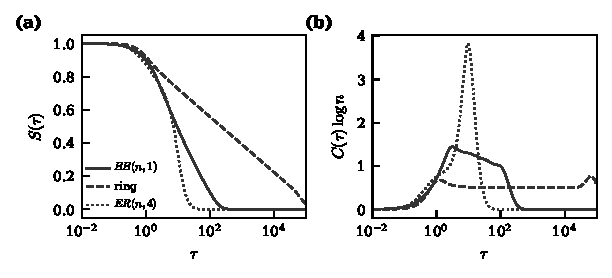
\includegraphics[width=\linewidth]{figs/fig-hc-entropy.pdf}
\caption{\textbf{The diffusion thermometer.} (a) Spectral entropy $S(\tau)$ and
(b) specific heat $C(\tau)\log n$, for a locally grown network, a ring and a random
network of a thousand nodes each. The ring's plateau at $0.5$ is its spectral
dimension of one, read off by Eq.~\eqref{eq:hc-plateau}; the random network's single
peak is its one and only characteristic scale.}
\label{fig:hc-entropy}
\end{figure}

Let a unit of something --- probability, heat, information --- spread over the
network by the diffusion equation $\dot{\mathbf{s}} = -L\mathbf{s}$, whose solution
is the propagator $e^{-\tau L}$. The single parameter $\tau$ is a \emph{diffusion
time}, and it doubles as a resolution: at small $\tau$ the spreading has not left
the immediate neighborhood of wherever it started, at large $\tau$ it has reached
everywhere and forgotten the difference.

The move that turns this into an instrument, due to \citet{villegas2023} and
building on the spectral-entropy formalism of \citet{dedomenico2016}, is to treat
the propagator as a statistical-mechanical density operator,
\begin{equation}
  \rho(\tau) = \frac{e^{-\tau L}}{\mathrm{Tr}\,e^{-\tau L}},
  \label{eq:hc-rho}
\end{equation}
which is the Boltzmann weight $e^{-\beta H}/Z$ with the Laplacian in the role of the
Hamiltonian and the diffusion time in the role of inverse temperature. Everything
statistical mechanics does to a Boltzmann weight can now be done to a network.

\begin{calculation}{entropy, specific heat, and the spectral dimension}
Let $\lambda_1=0\le\lambda_2\le\dots\le\lambda_n$ be the eigenvalues of $L$ and
\begin{equation}
  \mu_i(\tau) = \frac{e^{-\tau\lambda_i}}{\sum_j e^{-\tau\lambda_j}}
  \label{eq:hc-mu}
\end{equation}
the eigenvalues of $\rho(\tau)$. The normalized entropy and its logarithmic
derivative are
\begin{equation}
  S(\tau) = -\frac{1}{\log n}\sum_{i=1}^{n}\mu_i\log\mu_i,
  \qquad
  C(\tau) = -\frac{\mathrm{d}S}{\mathrm{d}\log\tau} .
  \label{eq:hc-SC}
\end{equation}
$S$ runs from $1$ at $\tau=0$, where every node is its own island and $\rho$ is the
identity over $n$, down to $0$ as $\tau\to\infty$, where diffusion has homogenized
everything. $C$ is the specific heat of the diffusion, and it is the quantity to
read, for the reason that makes specific heats useful everywhere else in physics:
\emph{it is flat where nothing is happening and it peaks where a scale is being
crossed}.

The flat value is not arbitrary either. On a structure whose diffusion is governed
by a spectral dimension $d_s$ --- meaning the density of Laplacian eigenvalues near
zero behaves as $\lambda^{d_s/2-1}$ --- the entropy falls logarithmically,
$S \simeq -(d_s/2)\log\tau/\log n + \text{const}$, so that
\begin{equation}
  C(\tau)\,\log n \;\longrightarrow\; \frac{d_s}{2} .
  \label{eq:hc-plateau}
\end{equation}
A constant specific heat is therefore not merely the absence of a scale; its
\emph{height} measures the dimension the diffusion sees. On a ring, $d_s=1$ and the
plateau should sit at $0.5$. Measured on a ring of a thousand nodes it sits at
$0.508$.
\end{calculation}

Figure~\ref{fig:hc-entropy} shows the instrument working on three networks chosen to
bracket the possibilities. The ring gives a broad flat plateau: a walk on a ring
crosses one scale after another with nothing distinguishing them, which is what a
one-dimensional object looks like. The random network gives a single sharp peak: it
has exactly one scale, the crossover from local to global, and once past it there is
nothing left. A locally grown network sits between the two, with a plateau and then
structure.


\section{Two renormalization groups on one lattice}
\label{sec:hc-rg}

\begin{figure}[!ht]
\centering
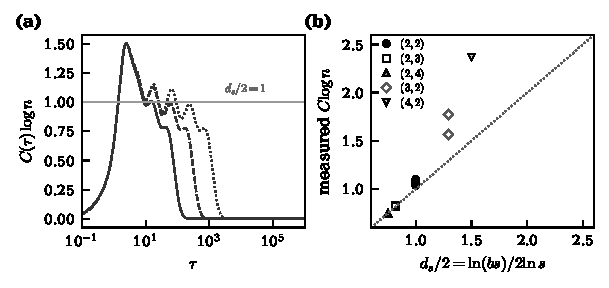
\includegraphics[width=\linewidth]{figs/fig-hc-diamond.pdf}
\caption{\textbf{A renormalization group read off a specific heat.} (a) The diamond
lattice at $b=s=2$ for three generations --- solid, dashed and dotted for $t=4$, $5$
and $6$, that is $n=172$, $684$ and $2732$. Each shows one peak per generation of the
construction, oscillating around the plateau $d_s/2=1$ that
Eq.~\eqref{eq:hc-plateau} predicts, with the ladder lengthening as the lattice
deepens. (b) Measured plateau against the prediction $\ln(bs)/2\ln s$ for the whole
$(b,s)$ family, diagonal dotted. The $b=2$ lattices sit on it; $b\ge3$ has not
converged at the sizes reachable by exact diagonalization.}
\label{fig:hc-diamond}
\end{figure}

On the diamond the instrument stops being descriptive and becomes exact, and the
reason is that this book already has a renormalization group for the same lattice.

Chapter~\ref{ch:communities} built one out of \emph{counting}: collect the block
statistics in a vector, and one generation of the construction acts on them by a
matrix whose two eigenvalues are $\lambda_{\mathrm{vol}}=bs$ for the interiors and
$\lambda_{\mathrm{seam}}=b$ for the boundary, so that the seam fades relative to the
bulk as $1/s$ per generation. That is a renormalization group on the description of
the network. The Laplacian renormalization group of \citet{villegas2023} is a
renormalization group on \emph{diffusion over} it: integrate out the fast modes,
rescale the time, repeat. Two flows, one object. They can be compared, and the
comparison has an answer.

\begin{calculation}{why one step is $s$ and the other is $s^{2}$}
One generation of the $(b,s)$ construction multiplies the pole-to-pole distance by
$s$ and the number of links by $bs$. Because $b$ parallel paths of $s$ links each
replace one link, the two-point resistance is multiplied by $s/b$. Diffusion time on
a resistive network goes as mass times resistance, so
\begin{equation}
  \tau \;\longrightarrow\; (bs)\cdot\frac{s}{b}\,\tau \;=\; s^{2}\,\tau .
  \label{eq:hc-tau-step}
\end{equation}
The walk dimension, defined by $\tau\sim \ell^{\,d_w}$ with $\ell\sim s$ the length
rescaling, is therefore
\begin{equation}
  d_w = \frac{\ln s^{2}}{\ln s} = 2
  \label{eq:hc-dw}
\end{equation}
identically --- for every $b$ and every $s$. The fractal dimension is
$d_f=\ln(bs)/\ln s$, and the spectral dimension follows as
\begin{equation}
  d_s = \frac{2 d_f}{d_w} = \frac{\ln(bs)}{\ln s} .
  \label{eq:hc-ds}
\end{equation}
So the two flows differ by exactly one power. The structural step rescales length by
$s$; the diffusive step rescales time by $s^{2}$, because on this lattice time is
length squared. And the two predictions the next paragraphs test are of different
robustness for a reason now visible: the spacing $s^{2}$ is governed by $d_w=2$,
which is independent of $b$, while the plateau height $d_s/2=\ln(bs)/2\ln s$ grows
with $b$, and a larger spectral dimension needs a larger lattice before its
small-$\lambda$ tail is resolved.
\end{calculation}

Both predictions are borne out, and the caveat the box anticipates is real.

\begin{center}
\footnotesize\setlength{\tabcolsep}{4pt}
\begin{tabular}{lrrrrrr}
\hline
$(b,s)$ & $t$ & $n$ & $d_s/2$ & $C\log n$ & peaks & $\tau$ ratio\\
\hline
$(2,2)$ & $3$ & $44$ & $1.000$ & $1.101$ & $1$ & --- \quad$(s^2{=}4)$\\
$(2,2)$ & $4$ & $172$ & $1.000$ & $1.069$ & $3$ & $4.4$ \quad$(s^2{=}4)$\\
$(2,2)$ & $5$ & $684$ & $1.000$ & $1.051$ & $4$ & $4.4$ \quad$(s^2{=}4)$\\
$(2,2)$ & $6$ & $2732$ & $1.000$ & $1.038$ & $5$ & $4.3$ \quad$(s^2{=}4)$\\
$(2,3)$ & $2$ & $30$ & $0.815$ & $0.824$ & $2$ & $5.3$ \quad$(s^2{=}9)$\\
$(2,3)$ & $3$ & $174$ & $0.815$ & $0.824$ & $3$ & $6.5$ \quad$(s^2{=}9)$\\
$(2,3)$ & $4$ & $1038$ & $0.815$ & $0.823$ & $4$ & $7.2$ \quad$(s^2{=}9)$\\
$(2,4)$ & $2$ & $56$ & $0.750$ & $0.746$ & $2$ & $10.2$ \quad$(s^2{=}16)$\\
$(2,4)$ & $3$ & $440$ & $0.750$ & $0.750$ & $3$ & $12.2$ \quad$(s^2{=}16)$\\
$(3,2)$ & $2$ & $23$ & $1.292$ & --- & $1$ & --- \quad$(s^2{=}4)$\\
$(3,2)$ & $3$ & $131$ & $1.292$ & $1.773$ & $1$ & --- \quad$(s^2{=}4)$\\
$(3,2)$ & $4$ & $779$ & $1.292$ & $1.566$ & $3$ & $4.0$ \quad$(s^2{=}4)$\\
$(4,2)$ & $2$ & $38$ & $1.500$ & --- & $1$ & --- \quad$(s^2{=}4)$\\
$(4,2)$ & $3$ & $294$ & $1.500$ & $2.368$ & $1$ & --- \quad$(s^2{=}4)$\\
\hline
\end{tabular}
\end{center}


\noindent Two kinds of entry are dashed rather than numbered, and neither is a
divergence. A spacing needs two peaks before it is a ratio at all, which is why the
shallowest lattices have none. And the plateau needs a scaling window to average over:
diffusion crosses the whole lattice at $\tau\sim s^{2t}$, so at $t=2$ that happens
before the spreading has escaped the smallest cell, the window closes on itself, and
there is simply no plateau to measure. Both are statements that the lattice is too
shallow to have the structure being looked for, which is the honest thing for the
instrument to say about two generations of anything.

\emph{The ladder.} The specific heat of the diamond is not a single peak
but a sequence of them, one per generation of the construction
(Figure~\ref{fig:hc-diamond}a): at $b=s=2$ there are three peaks at $t=4$, four at
$t=5$, five at $t=6$. A hierarchical lattice built by $t$ nested steps announces all
$t$ of them, at $t$ separate diffusion times. Their spacing converges on
Eq.~\eqref{eq:hc-tau-step} from above for $s=2$ --- $4.43$, $4.39$, $4.30$ against
$s^2=4$ --- and from below for the longer paths, $5.3$, $6.5$, $7.2$ against $9$ at
$s=3$, and $10.2$, $12.2$ against $16$ at $s=4$. The $(3,2)$ lattice at $t=4$ gives
$4.04$ against $4$. The spacing is the robust half of the prediction, as
Eq.~\eqref{eq:hc-dw} says it should be.

\emph{The height.} The plateau the ladder oscillates around is
Eq.~\eqref{eq:hc-plateau}, and for $b=2$ it is confirmed to within one per cent
across three values of $s$: at $(2,2)$ the measured $C\log n$ falls monotonically
through $1.101$, $1.069$, $1.051$, $1.038$ toward the predicted $1.000$ as the
lattice grows; at $(2,3)$ it sits at $0.823$ against a predicted $0.815$; at
$(2,4)$ it hits $0.750$ against a predicted $0.750$. For $b\ge3$ it does not
converge at reachable sizes --- $(3,2)$ reads $1.77$ then $1.57$ against $1.29$,
$(4,2)$ reads $2.37$ against $1.50$ --- moving the right way with size and not
arriving. Those two rows are reported as unconverged rather than as agreement.


The pseudofractal is the control that makes the ladder meaningful. It is built by a
recursion just as deterministic and just as self-similar as the diamond's, and it
has \emph{one} peak, at every generation tested --- $t=4$, $5$ and $6$ alike. There is
no ladder because there is no hierarchy of diffusion times to climb: the
pseudofractal's diameter grows like $\log n$ rather than like a power, so all its
scales collapse into one. Two deterministic self-similar lattices, both in this
book, and diffusion tells them apart at a glance where the community fits of
Chapters~\ref{ch:communities} to~\ref{ch:bubbles} put them in the same class.

\section{What the specific heat does not separate}

\begin{figure}[!ht]
\centering
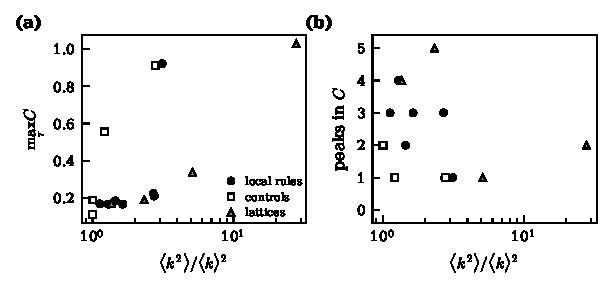
\includegraphics[width=\linewidth]{figs/fig-hc-rules.pdf}
\caption{\textbf{What the specific heat does not separate.} (a) Peak height and
(b) number of peaks against degree heterogeneity, one point per network. Locality
does not order either. The deterministic lattices of the previous section are
the exception.}
\label{fig:hc-rules}
\end{figure}

The diamond is the clean half of the story. Run the same instrument over the
stochastic rules and it is much less impressive, and that has to be said plainly,
because a specific heat is an easy thing to over-read once one has seen it work.

\begin{center}
\footnotesize\setlength{\tabcolsep}{4pt}
\begin{tabular}{lrrrrrr}
\hline
network & $n$ & $\langle k^2\rangle/\langle k\rangle^2$ & $C\log n$ & $\max C$ & peaks & flatness\\
\hline
\multicolumn{7}{l}{\emph{local rules}}\\
\quad $LS(n,1)$ & $1000$ & $1.64$ & $0.85$ & $0.17$ & $3$ & $0.38$\\
\quad $BB(n,1)$ & $1000$ & $2.75$ & $0.85$ & $0.21$ & $1$ & $0.55$\\
\quad $BB(n,2)$ & $1000$ & $1.45$ & $0.91$ & $0.18$ & $2$ & $0.31$\\
\quad $BB(n,3)$ & $1001$ & $1.29$ & $0.90$ & $0.17$ & $4$ & $0.13$\\
\quad $BB(n,5)$ & $1002$ & $1.13$ & $0.85$ & $0.17$ & $3$ & $0.17$\\
\quad $DS(n,0.5)$ & $1000$ & $2.70$ & $0.79$ & $0.22$ & $3$ & $0.71$\\
\quad $DD(n,0.5)$ & $1000$ & $3.13$ & $0.92$ & $0.92$ & $1$ & $1.85$\\
\multicolumn{7}{l}{\emph{controls}}\\
\quad $BA(n,2)$ & $1000$ & $2.79$ & $0.92$ & $0.91$ & $1$ & $1.79$\\
\quad $ER(n,4)$ & $986$ & $1.22$ & $0.87$ & $0.56$ & $1$ & $1.31$\\
\quad ring & $1000$ & $1.00$ & $0.51$ & $0.11$ & $2$ & $0.09$\\
\quad square lattice & $1024$ & $1.01$ & $0.77$ & $0.19$ & $2$ & $0.35$\\
\multicolumn{7}{l}{\emph{deterministic lattices}}\\
\quad pseudofractal & $1095$ & $5.13$ & $0.87$ & $0.34$ & $1$ & $0.98$\\
\quad rec.\ triangle & $768$ & $27.86$ & $0.93$ & $1.03$ & $2$ & $1.81$\\
\quad diamond $(2,2)$ & $2732$ & $2.33$ & $0.89$ & $0.19$ & $5$ & $0.36$\\
\quad diamond $(2,3)$ & $1038$ & $1.36$ & $0.81$ & $0.17$ & $4$ & $0.22$\\
\hline
\end{tabular}
\end{center}


\noindent What the specific heat does \emph{not} do is classify the growth rules. It
does not separate local from non-local: the peak height $\max_\tau C$ runs from
$0.17$ to $0.23$ across the bubble family and $LS(n,1)$, sits at $0.92$ for
duplication--divergence, and sits at $0.91$ for the non-local $BA(n,2)$ ---
duplication and preferential attachment landing on top of each other, which is the
one pairing this book most wants separated. Nor is it simply reading degree
heterogeneity, tempting as that looks: $BB(n,1)$ and $BA(n,2)$ have almost the same
$\langle k^2\rangle/\langle k\rangle^2$, $2.75$ against $2.79$, and differ by a
factor of four in $\max_\tau C$. And no peak of $C$ lands on the mean community size
$\langle n_B\rangle$ of Chapter~\ref{ch:graphons} for any rule, so the hope that a
specific heat would find the community scale for free is not fulfilled.

That is three things $C$ is not, and they are worth the space because the quantity
is easy to over-read. A peak in a specific heat is a scale, but a network may have
scales for reasons that have nothing to do with how it grew --- a broad degree
distribution will manufacture one --- and disentangling those on a stochastic rule is
beyond what this instrument does alone.


\section{Communities as compressed walks}

There is a third way to find communities in this book, and it belongs here rather
than in Chapter~\ref{ch:communities}, because its object is a walk.

Chapters~\ref{ch:communities} to~\ref{ch:bubbles} all minimize a description length,
and they all describe the same thing: the adjacency matrix. The map equation of
\citet{rosvall2008} minimizes one too, but of a \emph{random walk} on the network.
Name the modules, and a walk becomes a sequence of within-module codewords plus an
occasional module switch; a good partition is one that keeps that transcript short,
because the walker rarely leaves a module and so rarely pays for a switch. Compressing
the adjacency matrix asks where the links are; compressing a walk asks where the flow
goes, which depends on the links but also on how they compose into paths.

That gives the book three instruments for one question, and they are ordered by how
much dynamics they contain: the block model, which sees only the counts; the motif
alphabet of Chapter~\ref{ch:motifs}, which sees repeated wiring templates; and the
map equation, which sees where a walk gets stuck. Chapter~\ref{ch:bubbles} argued
that the first two are two currencies for one substance. Does the third buy the same
substance?

\subsection*{A test with a decisive pair}

The question has a clean experiment, because Chapter~\ref{ch:bubbles} supplies two
networks its two currencies treat oppositely. The pseudofractal --- $DBB(n,1)$, the
deterministic triangle rule --- has a footprint that tiles it completely: the alphabet
names $100\%$ of its links, and a fit with that alphabet then reports \emph{no}
communities at any size. Yet its meso-structure total $\kappa_0+\kappa$ still grows in
proportion to $n$, because the motifs are all there and all counted. $BB(n,1)$, the
stochastic version of the same triangle rule, has its footprint overlap itself: the
alphabet names $54\%$, and a genuine community residue is left over.

So the two hypotheses make opposite predictions. If the map equation buys the
meso-structure \emph{total}, it must find modules in both, since that total grows like
$n$ in both. If it buys the community \emph{residue}, it finds them only in the second.

\begin{center}
\footnotesize\setlength{\tabcolsep}{4pt}
\begin{tabular}{lrrrrrr}
\hline
 & & & \multicolumn{4}{c}{modules, by regularization strength}\\
network & $n$ & $m/n$ & none & $0.5$ & $1.0$ & $2.0$\\
\hline
pseudofractal $DBB(n,1)$ & $366$ & $1.99$ & $2$ & $26$ & $\mathbf{1}$ & $1$\\
pseudofractal $DBB(n,1)$ & $1095$ & $2.00$ & $6$ & $61$ & $\mathbf{1}$ & $1$\\
pseudofractal $DBB(n,1)$ & $3282$ & $2.00$ & $15$ & $160$ & $\mathbf{1}$ & $1$\\
diamond $(2,2)$ & $684$ & $1.50$ & $7$ & $45$ & $\mathbf{1}$ & $1$\\
diamond $(2,2)$ & $2732$ & $1.50$ & $12$ & $167$ & $\mathbf{1}$ & $1$\\
$BB(n,1)$ & $400$ & $1.99$ & $4$ & $30$ & $\mathbf{1}$ & $1$\\
$BB(n,1)$ & $1200$ & $2.00$ & $2$ & $81$ & $\mathbf{74}$ & $1$\\
$BB(n,1)$ & $3600$ & $2.00$ & $4$ & $220$ & $\mathbf{221}$ & $1$\\
$BB(n,2)$ & $1200$ & $1.50$ & $3$ & $102$ & $\mathbf{1}$ & $1$\\
$BB(n,2)$ & $3600$ & $1.50$ & $5$ & $283$ & $\mathbf{277}$ & $1$\\
ring $C_n(1)$ & $1200$ & $1.00$ & $5$ & $165$ & $\mathbf{1}$ & $1$\\
ring $C_n(1)$ & $3600$ & $1.00$ & $9$ & $413$ & $\mathbf{1}$ & $1$\\
ring $C_n(1,2)$ & $1200$ & $2.00$ & $4$ & $111$ & $\mathbf{111}$ & $1$\\
ring $C_n(1,2)$ & $3600$ & $2.00$ & $7$ & $291$ & $\mathbf{291}$ & $1$\\
ring $C_n(1,2,3)$ & $1200$ & $3.00$ & $3$ & $88$ & $\mathbf{87}$ & $1$\\
\hline
\end{tabular}
\end{center}


\noindent The residue wins, and not narrowly. On the pseudofractal the map equation
returns a single module at every size tested, up to $n=3282$; on the diamond, the other
lattice the alphabet names completely, the same. On $BB(n,1)$ it returns one module at
$n=400$ and then $74$ and $221$ at $n=1200$ and $3600$ --- a constant density of about
$0.06$ per node once past an onset. $BB(n,2)$ does the same with a later onset. The map
equation is tracking $\kappa$ and not $\kappa_0+\kappa$: it reports nothing on exactly
those networks whose structure a blueprint can stamp out, even though the structure is
demonstrably there.

The rings sharpen that, and they are the control Chapter~\ref{ch:communities} supplies
for free. That chapter proves the ring is split by a block model exactly when its links
outnumber its nodes --- when it carries an extensive number of independent cycles. The
map equation agrees on the ring family: $C_n(1)$, sitting at $m/n=1$, gives one module;
add second neighbours and $C_n(1,2)$ at $m/n=2$ gives $111$ and $291$ modules at $n=1200$
and $3600$; third neighbours keep it there. Two instruments with almost nothing in
common, drawing the same threshold on the same family.

But the pseudofractal also has $m/n \to 2$, and it has no modules. So an excess of links
over nodes is necessary and not sufficient, and the missing ingredient is what the map
equation is actually sensitive to. A walk gets stuck only where there is a
\emph{bottleneck}. The ring's excess links leave long arcs with narrow cuts between
them; the pseudofractal's excess links are triangles, which are structure without being
a barrier to anything, laid over a lattice whose hubs put every node within
$\log n$ steps of every other. Meso-structure and bottleneck are not the same property,
and the map equation is a bottleneck detector wearing a description length.

One caveat has to be stated because the numbers move with it. Infomap here is
regularized, and the regularization strength matters: at $0.5$ every network in the
table fragments, the pseudofractal included, into a few per cent of $n$ modules, and at
$2.0$ every one of them collapses to a single module. The discrimination reported above
exists at strength $1.0$. That value is not chosen to produce it --- it is the library's
default, and the setting under which communities in $BB(n,1)$ were reported in the first
place \citep{vazquezcommunities2025} --- but the finding is a statement about the default
regularization rather than a parameter-free fact, and a reader should hold it that way.

There is a last thing worth noticing, and it belongs to the next chapter as much as
this one. The pseudofractal, on which compressing a walk finds no structure at all, is
the network on which Chapter~\ref{ch:quantum} finds a \emph{quantum} walker more tightly
trapped than anywhere else in this book --- confined to under four nodes. A classical
walker needs a bottleneck to be trapped and there is none; a quantum walker can be
trapped by interference, and the triangles supply that in abundance. The same lattice,
two walkers, opposite verdicts. Which is the sharpest available statement of what the
next chapter adds.

\section{What the classical walker misses}

Two things are now on the table, and the next chapter needs both.

The first is that diffusion is a real instrument. It recovers the spectral dimension
of a ring and of a whole family of hierarchical lattices from nothing but a
spectrum; it counts the generations of a construction; and it does all of that with
no partition to infer, no prior to choose and no vocabulary to fix ---
Chapter~\ref{ch:bubbles}'s objection about description length does not apply to it
at all. That is worth having on its own.

The second is what it costs. A classical walk is \emph{irreversible}: it relaxes,
and Eq.~\eqref{eq:hc-SC} is a statement about how it relaxes. The entropy $S(\tau)$
is monotone, running from one to zero, and once it has reached zero the walk has
forgotten everything, including where it began. Everything this chapter measured is
therefore a property of the \emph{approach} to that forgetting --- how fast, through
what scales, in what order. There is no regime in which a classical walker simply
declines to spread.

Chapter~\ref{ch:quantum} removes exactly that. Replace the diffusion equation with
the Schr\"odinger equation and the evolution becomes unitary: nothing relaxes,
nothing is forgotten, and a walker can be confined for all time rather than merely
delayed. The specific heat of this chapter measures the scales on the way to
equilibrium; the localization volume of the next measures a walker that never gets
there. It is the same operator $L$ in both, which is what makes the pair worth
having.

\section{Summary}

A random walk's stationary distribution knows a network's degrees and nothing else,
and its mean return time $2m/k_i$ is exactly as blind --- but its transient behaviour
is not, and the mean first passage time between two nodes is a global quantity whose
asymmetry defines a centrality that degree cannot see. Treating the diffusion
propagator $e^{-\tau L}$ as a Boltzmann weight turns the diffusion time into a
resolution knob and gives a spectral entropy and a specific heat, where a flat
specific heat means no characteristic scale and its height measures the spectral
dimension the diffusion sees: $0.508$ against an exact $0.5$ on a ring. On the
diamond lattice the instrument becomes exact and meets the renormalization group
Chapter~\ref{ch:communities} built by counting. The two differ by one power, for a
reason that can be derived: the structural flow rescales length by $s$ while the
diffusive flow rescales time by $s^2$, because the walk dimension of this lattice is
two for every $b$ and $s$. The specific heat then shows one peak per generation of
the construction, spaced by $s^2$, oscillating around a plateau at
$\ln(bs)/2\ln s$ --- confirmed to one per cent for $b=2$ across three path lengths,
and unconverged for $b\ge3$. The pseudofractal, self-similar by an equally
deterministic recursion, has one peak and no ladder, because its scales collapse
into a logarithm. What the specific heat does \emph{not} do is classify the
stochastic rules: it puts duplication and preferential attachment on top of each
other, and none of its peaks finds the community size. And a classical walk always
relaxes in the end, so everything here measures the approach to forgetting rather than
any refusal to spread.
